%%%%%%%%%%%%%%%%%%%%%%%%%%%%%%%%%%%%%%%%%%%%%%
%                insertmeeting
% 1) Title (something creative & funny?)
% 2) Date (MM/DD/YYYY)
% 3) Location (ex. Hagerty High School)
% 4) People/Committees Present 
% 5) Picture 
% 6) Start Time & Stop Time (ex. 12:30AM to 4:30PM)
%%%%%%%%%%%%%%%%%%%%%%%%%%%%%%%%%%%%%%%%%%%%%%
\insertmeeting 
	{Autonomous Accidents} 
	{01/14/22} 
	{Hagerty High School}
	{Annika, Anouska, Clayton, Falon, James, Jensen, Nathan, Ritam, Rose, Samantha}
	{Images/RobotPics/robot.jpg}
	{2:30 - 4:30}
	
\hhscommittee{Software}
\noindent\hfil\rule{\textwidth}{.4pt}\hfil
\subsubsection*{Goals}
\begin{itemize}
    \item Continue refining autonomous for the blue alliance 

\end{itemize} 

\noindent\hfil\rule{\textwidth}{.4pt}\hfil

\subsubsection*{Accomplishments}
Our first priority for today was to refine the autonomous program for the blue alliance. We started with the program for retrieving the blocks when we started far from the carousel. Previously, we were running into problems with the robot going the incorrect distance when moving to the blocks. We just kept trying different distances until the robot moved to the correct location. We finally realized that we could change the maxOutput of the drivebase, giving us greater control of the robot's motion. The next portion that we tackled was to divide the parking portion of the program into two parts - GO TO PARK 1 and GO TO PARK 2. This allowed us to keep a park state consistent for both the red and blue sides, while adjusting for the different actions needed in GO TO PARK 2. 
 
\begin{figure}[htp]
\centering
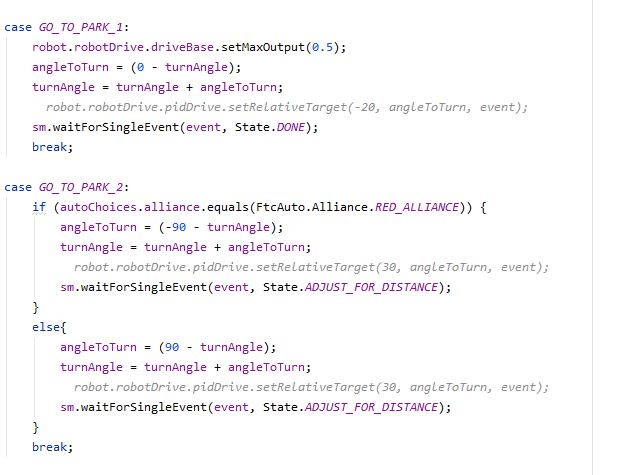
\includegraphics[width=0.95\textwidth, angle=0]{Meetings/January/01-14-22/1.14.22 fixed park into 2 parts - James Hu.JPG}
\caption{Splitting the park portion into two parts}
\label{fig:011422_1}
\end{figure}

\whatsnext{
\begin{itemize}
    \item Continue to improve autonomous, specifically for the blue alliance far from carousel. 
\end{itemize} 
}

